% % Created 2015-09-15 Tue 11:46
% \documentclass[11pt]{article}
% \usepackage[utf8]{inputenc}
% \usepackage[T1]{fontenc}
% \usepackage{fixltx2e}
% \usepackage{graphicx}
% \usepackage{longtable}
% \usepackage{float}
% \usepackage{wrapfig}
% \usepackage{rotating}
% \usepackage[normalem]{ulem}
% \usepackage{amsmath}
% \usepackage{textcomp}
% \usepackage{marvosym}
% \usepackage{wasysym}
% \usepackage{amssymb}
% \usepackage{hyperref}
% \usepackage{color}
% \usepackage{soul}
% \tolerance=1000
% \usepackage[margin=1in]{geometry}

% \newcommand{\hilight}[1]{\colorbox{yellow}{#1}}

% %\author{Alex Ansari}
% %\date{}
% %\title{TALOS}
% %\hypersetup{
% %  pdfkeywords={},
% %  pdfsubject={},
% %  pdfcreator={Emacs 24.3.1 (Org mode 8.2.10)}}


% \begin{document}
\section{IHMC Mobility Assist Exoskeleton (MAE)}
\label{ihmc}
\begin{refsection}[exos/ihmc.bib]

Although the IHMC MAE was primarily designed as a disabled assist exoskeleton, the device is also provides a ``performance enhancement" control mode, which is within the scope of this document.  The main design principle highlighted in the IHMC MAE hardware (a recurring theme throughout exoskeleton literature) is that directly measuring user intent can be difficult for a number of reasons.  The IHMC designers resolve the issue using a new control and feedback system, which for the IHMC MAE, is primarily based on a unique actuation scheme. 

The IHMC MAE uses novel series elastic actuators (SEAs) in their hardware design mostly because they offer the ability to perform high-fidelity impedance control.  In series elastic actuators, a compliant element is placed in series after the output a motor's drive mechanism. The measured compression of the compliant element is used to calculate the force, or torque, acting on the output of the actuator.  { \bf Series elastic actuators} are generally viewed as a good way to provide {\bf accurate force feedback} information and to provide a {\bf low mechanical impedance}.  The major disadvantage of SEAs is that they have a relatively low bandwidth at high forces, as the compliant element needs time to compress before a force can be sensed and thus inherently include a delay between the time a force is applied and when the control system can react.


\subsection{Actuator specifications}

The IHMC actuators are designed based on data collected from clinical gait analysis.  Specifically, the actuators at the hip and knee were designed to be able to provide 40Nm of peak torque during the stance phase of the walking gait cycle.  The rotary SEA is composed of a Moog BN34-25EU-02 brushless DC motor with a 1:100 harmonic drive (SHD-20).  
 
The spring mechanism, which sits between the gearbox and joint output, is shown in Figure \ref{fig:IHMCSEA}.  The mechanism uses linear die springs and an angular encoder to measure the joint torque output.  The choice of linear die spring was based on the spring's predictable force to displacement function as well as favorable energy storage to weight characteristics.  
\begin{figure}[thpb]
\centering
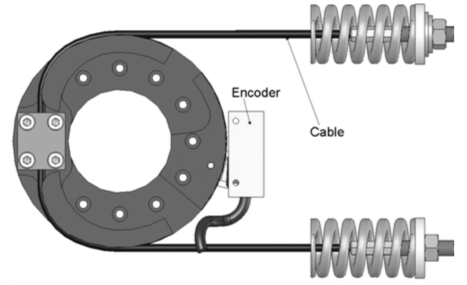
\includegraphics[width=3.in]{exos/figs/ihmc/seaAssm}
  \caption{Schematic of the RSEA elastic mechanism design, shown in the zero force position. The encoder reads a scale tape on the curved cylindrical surface. Note that the actuator housing and bearing have been omitted for clarity.}
%  \vspace{-0.2in}
 \label{fig:IHMCSEA}   
 \end{figure}
 
Fully assembled, the actuator has a  {\bf torque limit of 80 Nm}, with a {\bf velocity limit of 6.8 rad/s}.  As noted, the {\bf bandwidth of the actuator} is its primary drawback, which limits the torque control to approximately {\bf 10 Hz at amplitudes greater than 15 Nm} and up to {\bf 30Hz for lower magnitude forces}. 
 
 \subsection{Exoskeleton Specifications}
 
 The IHMC MAE lower extremity exoskeleton includes a total of ten degrees of freedom (DOF), six of which are active and four are passive.  Five DOF correspond to the two legs of the system.  Each of the powered joints is powered using the SEA joint discussed in the previous subsection.  A labeled diagram of the IMHC system is shown in Figure \ref{fig:IHMCSYS}.  
 
 The hip ad/abduction as well as flexion/extension DOFs are actively actuated.  The hip yaw DOF consists of a curved spring-loaded roller bearing whose center of rotation is approximately at the user's hip joint. The knee flexion/extension joint is connected to the hip flexion/extension joint using telescoping tubes and is also actuated.  The final DOF is the dorsal flexion at the ankle joint.  This joint is spring loaded such that it provides unidirectional torque for toe clearance during walking.
 
 In its current configuration, the IHMC exoskeleton in controlled by an off-board computer and is powered using a tether. The suit {\bf includes position and force sensors in the actuators in addition to two foot switches per foot}.  The foot switches are used to detect whether the system is in single or double support phase.  It also provides information used to estimate the load distribution to the stance legs.
 
 
 \begin{figure}[thpb]
\centering
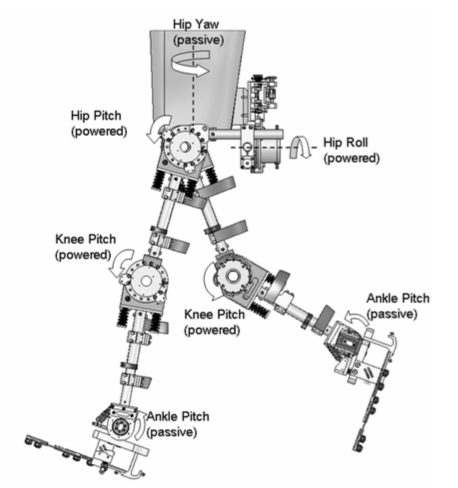
\includegraphics[width=3.in]{exos/figs/ihmc/ihmcSys}
  \caption{Side view of the IHMC Mobility Assist Exoskeleton showing the powered and passive degrees of freedom.}
%  \vspace{-0.2in}
 \label{fig:IHMCSYS}   
 \end{figure}
 
 
 \subsection{Control Specifications}
 
 Both IHMC MAE control approaches noted are relatively straight forward implementations of low-level torque control.  The first control scheme takes full advantage of the SEA actuators' ability to directly measure output torque and subsequently to perform closed-loop torque control, (see Fig~\ref{fig:IHMCTOR}). 
  \begin{figure}[thpb]
\centering
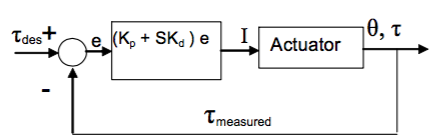
\includegraphics[width=3.in]{exos/figs/ihmc/torqueCon}
  \caption{Torque control loop in the actuator control system.}
%  \vspace{-0.2in}
 \label{fig:IHMCTOR}   
 \end{figure}
 The controller takes in a desired torque, compares the desired value to the output torque measured at each individual actuator, then uses this value as well as its derivative to compute an actuator command signal, which in this case is a current.  The largest question in this controller, as presented in literature, is how to define the desired torque term $\tau_\text{des}$.
 
 The second low-level control approach presented in the IHMC MAE literature is a combination of a position-based controller with an inner-loop torque controller.  This control scheme is presented in Figure \ref{fig:IHMCPOS}.
  \begin{figure}[thpb]
\centering
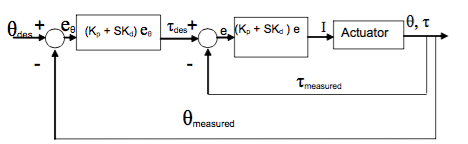
\includegraphics[width=3.in]{exos/figs/ihmc/positionCon}
  \caption{Control system diagram for an actuator. The torque feedback is fed to an inner control loop while the position is fed back to the overall position controller.}
%  \vspace{-0.2in}
 \label{fig:IHMCPOS}   
 \end{figure}
 The controller in Figure \ref{fig:IHMCPOS} shows an outer-loop position-based PD controller that takes in desired joint trajectories and compares them to measured joint positions.  These are used to generate desired torque values which are fed into an inner closed-loop torque control loop.  This control scheme is a good low-level choice if high-impedance. accurate suit motion is desired.  Similarly to the torque-only control loop above, the main question in this control scheme is how to obtain the desired joint trajectories.  
 
 One possibility for defining either the desired torques / joint trajectories in these control schemes is to use clinical gait analysis data.  With this approach, the highlighted controllers would effectively play back nominal joint trajectory data.  The foot sensors in the system would detect phase transitions, allowing the controllers to dynamically adjust the prerecorded data to the user in realtime.
 
 
 \subsection{Assessment and Recommendations}
 
The design of the IHMC MAE is in many ways centered around being able to perform high-fidelity force control.  In general we support the ability to perform force control using a direct measurement (or near direct) of the force/torque at the output of the transmission system.  Series-elastic actuators may provide a solution to this problem for a number of operational scenarios, but caution should be taken when considering this solution for highly dynamic behaviors, as the control bandwidth at the actuator may be too slow to safely react in dynamically changing environments. 
 
One potential other issue with the IHMC control design is that they only appear to address low-level control.  The designers have not specified how to generalize the process of generating torque / joint reference trajectories, in other words there is a lack of information with respect to the typical ``mid-level" of a hierarchical control scheme.  Thus combining other approaches with the low-level, highly accuracy torque control provided by the novel SEAs presented in this section could offer a potentially beneficial control solution.
 
All of the figures as well as hardware and control specifications in this section are taken from \cite{ihmc_2009}.
 
\printbibliography[heading=subbibliography]

\end{refsection}


% \end{document}


% Hian Kai Kwa and Jerryll H. Noorden and Mathew Missel and Travis Craig and Jerry E. Pratt and Peter D. Neuhaus, "Development of the IHMC Mobility Assist Exoskeleton,"  International Conference on Robotics and Automation, 2009.



%%% Local Variables:
%%% mode: latex
%%% TeX-master: "../survey"
%%% End:
